\documentclass[format=sigconf]{acmart}
\settopmatter{printacmref=false} % Removes citation information below abstract
\renewcommand\footnotetextcopyrightpermission[1]{} % removes footnote with conference information in first column
\usepackage[utf8]{inputenc}
\usepackage{amsmath}
\usepackage{hyperref}
\usepackage{makecell}

\settopmatter{printacmref=false}

\title{Mathematical model approach for draft picking in basketball}

\author{Lawrence Thanakumar Rajappa}
\affiliation{\institution{IDA Linköping University}}
\email{lawra776@student.liu.se}

\date{December 2020}
\begin{document}
\maketitle
\pagestyle{plain} % Remove ACM page header

\section{Introduction}
Analytics is being used in all fields such as healthcare, manufacturing, banking and etc. for decision-making. Likewise, 
analytics is also playing a major role in Sports industry such as football, baseball, basketball and etc. to predict player's 
next move, injury analysis, position analysis and etc. Sports analytics is being spoken as a concept for many years which 
could be used to improve team performance, as a result, the revenue generation is very much improved for the team. For this 
project, we will mostly focus on basketball. In order to have a good prediction and analysis report, we need to have proper
dataset and most importantly, the data must also have most important attributes that could provide insights for a given problem.

There are many ways that the data can be used by the team for various purposes. The kind of data that the team would use includes
average stats of the players, per game stats, and etc. These data can be used to understand a player in terms of strengths and 
weaknesses, emotional stability and etc. These attributes could be used to assess the team's performance. Moreover, there are other 
attributes such as weather conditions, the condition of the field and even psychological factors such as the fans support should be
included along with player's data to determine the team's performance. This document speaks about how the data are being used by
a basketball team to select players using mathematical models.

\section{Aim}
In this project, the aim is to create a draft picking system for a basketball team by using 3 mathematical models namely, model 1 : model
to predict whether a player will stay in the team for five years or not, model 2: model to determine the position of players 
based on their previous experiences and model 3: model to cluster or group players based on previous performances. These models
would facilitate team managers and coaches to select players and make best out of them.

\section{Motivation}
Before the advent of analytics, the selection of players or draft formation was done manually which was a time consuming and huge 
workload. The emergence of analytics and computing resources has paved a new way in recruiting best players based on their previous
performances in a short period of time with minimal workload. However, Sports industry has restricted for the complete adoption of 
analytics into their respective teams because teams spend three-fourth of their revenue for paying salaries to the players
and to cover other expenditures. Hence, the teams cannot afford to invest huge sum of money in technology, data and analytical 
tools  \cite{davenport2014analytics}. This project would remove the above mentioned bottleneck and facilitate the teams to use 
analytical tools with much lower cost and at ease. 

\section{Earlier system}
Earlier to 2005, the data was collected by a person watching the game using either a notepad and pen or black boards with chalks.
This data was prone to human errors. As a result, the analysis carried out on this data and results were misleading.
In 2005, two Isareli scientists, Gal Oz and Miky Tamir, created a system called \textit{SportsVU} (see in figure \ref{fig:SportsVU})
\cite{mccann2012player} \cite{warsaw}. This
system captures the ball movement as well as athletes movement, all these data are combined together for statistial analysis using 
the statistical algorithms that the company has created \cite{warriors}.
Based on the statistial analysis inference, the players were chosen for a team, but this method was manual. Moreover, other data such 
as Rebounds, TurnOver and etc were calculated from this system as well as from manually gathered data.

\begin{figure}[H]
    \centering
    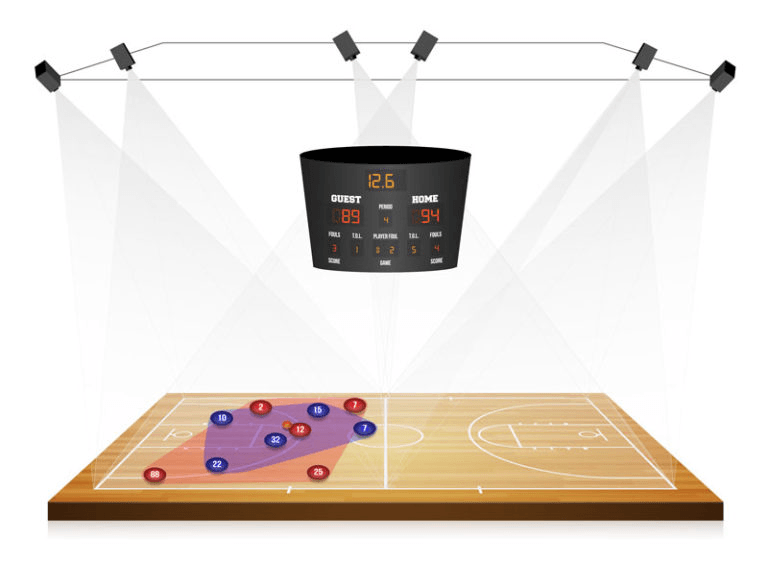
\includegraphics[scale=0.20]{STATS-SportVU-technology.png}
    \caption{SportsVU in basketball court.}
    \label{fig:SportsVU}
\end{figure}

\section{Background}
In this part, some general terms that are relative to the topic are going to be discussed. It is important to understand them for further
reading. 

The terms that will be discussed are:
\begin{itemize}
    \item  Draft picking and its process.
    \item  Machine learning.
    \item  Sports Analytics.
\end{itemize}
\subsection{Draft picking and its process}
NBA draft is an annual event where basketball teams select players from american colleges and from international professional league
for their rosters. Once a team selects a player, then the team has right to sign a NBA contract with the player.

In draft picking process, teams select eligible players in turns. There are two rounds in the draft where all 30 teams participate
to select a player in turns, meaning every year 60 eligible players are drafted, but teams that did not reach the playoffs 
in the previous regular season or teams with worst performs selects a player by undergoing a process called \textit{NBA Draft Lottery}.
This process determines the selection order of the team or provides an opportunity for the team which wins the lottery to pick the
first draft followed by other worst performing teams. The team with best records receives the 30\textsuperscript{th} pick. During the
second round in the draft, there is no lottery system, but teams pick the draft in the reverse order based on the previous regular 
season's standings. Moreover, the teams can exchange their draft picks with each other, for example, in 2019 the Minnesota Timberwolves 
traded the No. 11 pick and forward Dario Saric to the Phoenix Suns in exchange for the No. 6 pick. But, there are some restrictions
based on \textit{The Stepien Rule}, that is, this rule prevents the team from trading their first-round draft pick in consecutive 
years \cite{draft}.

\subsection{Machine learning}
Machine learning is a general concept and broader area which consists of many definitions provided by recognized and reliable 
universities, institutions, professors and organizations and they are as follows,
\begin{itemize}
    \item "Machine learning is based on algorithms that can learn from data without relying on rules-based programming." \cite{machineLearning1}
    \item "The field of Machine Learning seeks to answer the question “How can we build computer systems that automatically 
           improve with experience, and what are the fundamental laws that govern all learning processes?" \cite{machineLearning2}
    \item and etc.
\end{itemize}
\begin{figure}[H]
    \centering
    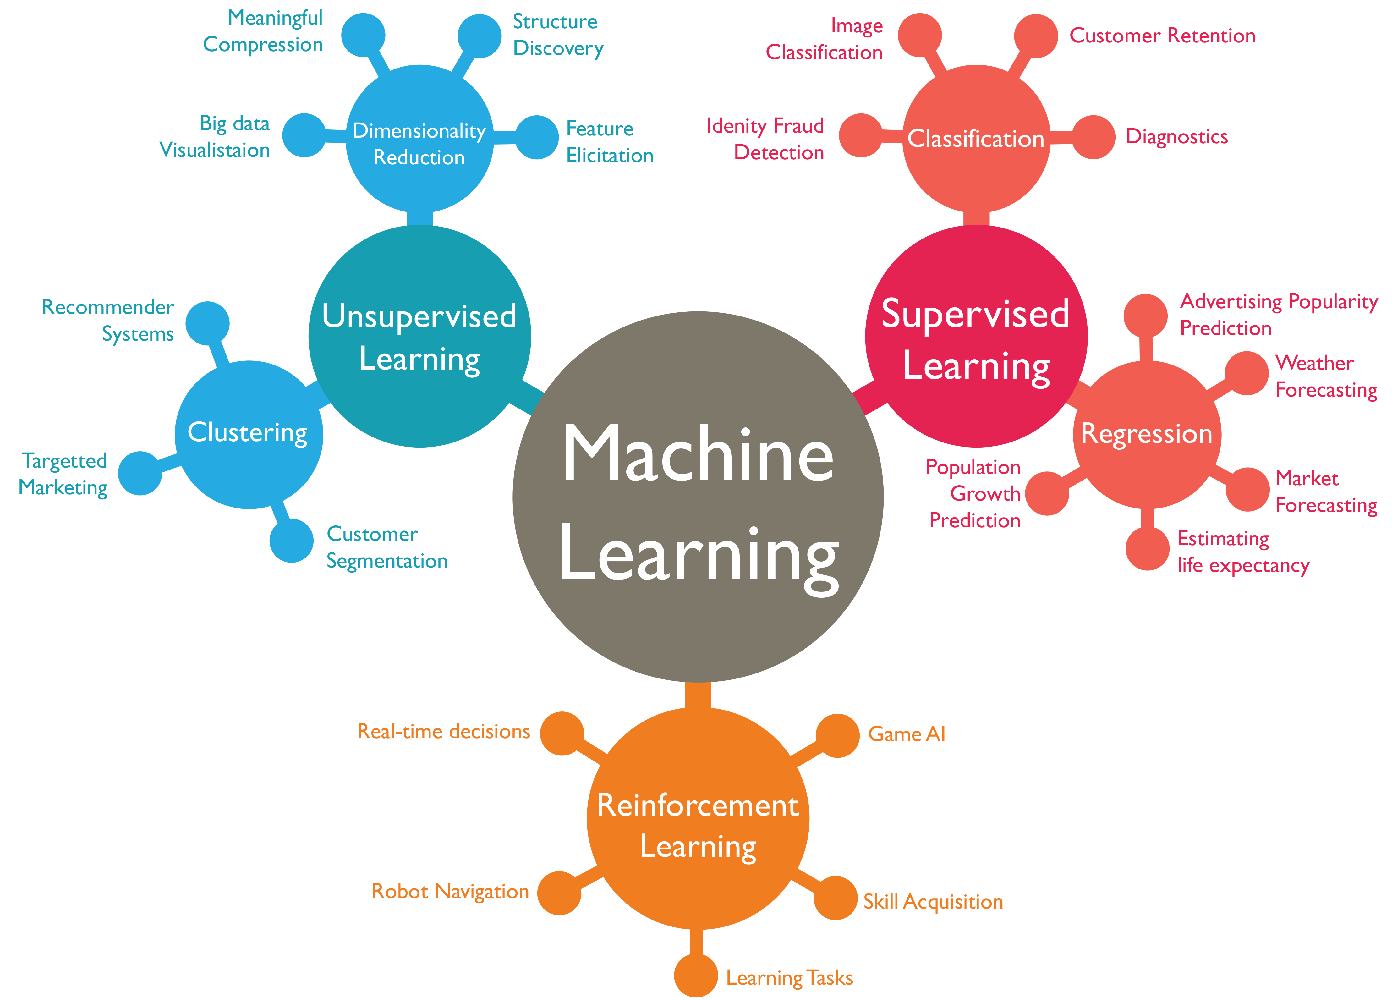
\includegraphics[scale=0.70]{Machine_Learning.png}
    \caption{Machine Learning in an eagle view}
    \label{fig:ml}
\end{figure}
Machine learning can be categorized in three types,
\begin{itemize}
    \item Supervised Learning.
    \item Unsupervised Learning.
    \item Reinforcement Learning.
\end{itemize}
The definitions for the above terms are:
\begin{itemize}
    \item "Supervised learning algorithms generate a function that maps inputs to desired outputs, based
    on a set of examples with known output (labeled examples)" \cite{tzanis2009machine}.
    \item "Unsupervised learning algorithms find patterns and relationships over a given set of inputs 
    (unlabelled examples)" \cite{tzanis2009machine}.
    \item "Reinforcement learning, where an algorithm learns a policy of how to act given an observation of the world" \cite{tzanis2009machine}.
\end{itemize}
In this project, we will mostly focus on Supervised and Unsupervised learning algorithms. The different types of algorithms in both
supervised and unsupervised learning are given below, \\

Some algorithms of supervised learning:
\begin{itemize}
    \item Nearest Neighbor
    \item Naive Bayes
    \item Support Vector Machine (SVM)
    \item Logistic Regression
    \item Linear Regression
    \item and etc.
\end{itemize}
\par
Some algorithms of unsupervised learning:
\begin{itemize}
    \item k-means clustering
    \item Association Rules \cite{typeofml}
    \item and etc.
\end{itemize}
\subsection{Sports Analytics}
Sports analytics is the application of above mentioned algorithms to sport in order to draw useful insights which could help 
an individual athlete's performance, or a team's performance for a season. It can also help teams to perform injury analysis
and steps to mitigate them, salary of a player based on his previous performances and etc. Nowadays,  many teams, coaches and 
even players are adopting sports analytics for decision making.

"The analytics split nicely between the front-office and back-office. Front-office analytics
include topics like analyzing fan behavior, ranging from predictive models for season ticket
renewals and regular ticket sales, to scoring tweets by fans regarding the team, athletes,
coaches, and owners. This is very similar to traditional customer relationship management.
Financial analysis is also a key area, especially for the pros where salary caps or scholarship
limits are part of the equation. Back-office uses include analysis of both individual athletes as
well as team play. For individual players, there is a focus on recruitment models and scouting
analytics, analytics for strength and fitness as well as development, and predictive models for
avoiding overtraining and injuries. Concussion research is a hot field. Team analytics include
strategies and tactics, competitive assessments, and optimal roster choices under various onfield or on-court situations.” \cite{tichy2016changing}
\begin{figure}[H]
    \centering
    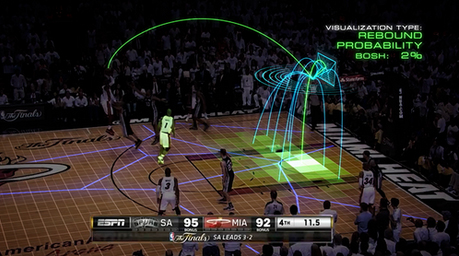
\includegraphics[scale=0.50]{sportsanalytics.jpg}
    \caption{Sports Analytics}
    \label{fig:sa}
\end{figure}
However, the analytical methods and data has to be kept safe and should be extremely careful because the data and methodology
could lead to numerous problems such as issues with betting companies, non-ethical training of atheletes leading to injuries and 
etc. \cite{spa}
\section{Methodology}
This section describes the framework used for draft picking in basketball using Machine learning. The proposed framework consists of 
3 mathematical models namely career longevity model, providing positions to selected players and grouping players based on their 
performance into two groups, either 1 or 0. Initially, the user or the coach or the team manager loads the players data to \textbf{model 1},
which provides list of players who will stay with the league for more than 5 years and list of players who don't stay for more than
5 years. This output is provided as an input to \textbf{model 2} which predicts the positions of the players based on previous 
performance. Finally, the output of 2\textsuperscript{nd} model is provided as an input to the \textbf{model 3} where players are 
grouped as 1 and 0, that is, either good or bad pick. This proposed framework is time efficiency, environmental friendly (less 
paperwork) and user friendly.

Subsection \textbf{6.1} describes the libraries or functions used in the proposed framework. Subsection \textbf{6.2} descibes about the 
source of data, structure of data, and pre-processing of data. Subsection \textbf{6.3} describe both supervised and unsupervised 
learning algorithms which are used to create 3 mathematical models for draft picking. The framework applies many algorithms and 
chooses one algorithm which performs better than the other algorithms for each model. This section concludes 
with Subsection \textbf{6.4}, which describes the evaluation metrics used.

\subsection{Libraries}
The following Python programming packages or libraries have been used by the proposed framework for data pre-processing and model building,
\begin{itemize}
    \item NumPy for numerical computations.
    \item Pandas for data loading.
    \item MatplotLib and Seaborn for visualization.
    \item sklearn for evaluation metrics and model building (Supervised and Unsupervised learning).
    \item Pickle for loading and saving of data objects, mathematical model objects and etc.
    \item statsmodel for checking  multicollinearity in data.
\end{itemize}
\subsection{Dataset}
\subsubsection{Source of data}
\hfill\\
The two main sources for dataset used by the proposed framework are,
\begin{itemize}
    \item \href{https://www.basketball-reference.com/}{basketball-reference.com}
    \item \href{https://data.world/}{Data.world}
\end{itemize}
\par
The data provided by Basketball-reference.com contains the NBA players overall performance such as rebounds, turnovers, points, games 
played and etc. for a regular season which can be either web scrapped or downloaded in comma-separated format file (CSV). Data.world
provides NBA players data such as players demographic data, players salary data and etc. which are less in number. By combining data
from both sources, yields a large dataset required for model building.

\subsubsection{Structure of data}
\hfill\\
The dataset contains players performance with the following main attributes,
\begin{center}
    \begin{table}[H]
        \begin{tabular}{|c|c|}
            \hline
            \textbf{Attributes} & \textbf{Descriptions} \\
            \hline
            GP & Games Played \\
            \hline
            POS & Position \\
            \hline
            MP & Minutes Played \\
            \hline
            PTS & Points \\
            \hline
            FG & \makecell{Field Goals (both 2 point field goals \\ and 3 point field goals)} \\
            \hline
            FGA & \makecell{Field Goal Attempts (includes both 2-point \\ field goal attempts and \\3-point field goal attempts)} \\
            \hline
            FG\% & Field Goal Percentage; the formula is FG / FGA. \\
            \hline
            3P & \makecell{3-Point Field Goals (available since \\the 1979-80 season in the NBA)} \\
            \hline
            3PA & \makecell{3-Point Field Goal Attempts (available since \\the 1979-80 season in the NBA)} \\
            \hline
            3P\% & \makecell{3-Point Field Goal Percentage (available since \\the 1979-80 season in the NBA); \\the formula is 3P / 3PA.}\\
            \hline
            FT & Free Throws \\
            \hline
            FTA & Free Throw Attempts \\
            \hline
            FT\% & Free Throw Percentage; the formula is FT / FTA\\
            \hline
            ORB & Offensive Rebounds \\
            \hline
            DRB & Defensive Rebounds \\
            \hline
            TRB & Total Rebounds \\
            \hline
            AST & Assist \\
            \hline
            AST\% & \makecell{Assist percentage \\the formula is 100 * AST / (((MP / (Tm MP / 5))\\ * Tm FG) - FG).
            Assist percentage is an estimate of the \\percentage of teammate field \\goals a player assisted while he was on the floor.} \\
            \hline
            STL & Steal \\
            \hline
            BLK & Block \\
            \hline
            BLK\% & \makecell{Block Percentage \\ the formula is 100 * (BLK * (Tm MP / 5)) /\\ (MP * (Opp FGA - Opp 3PA)) \\
            Block percentage is an estimate of the percentage of \\opponent two-point field goal attempts blocked\\ by the player while he was on the floor}\\
            \hline
            TOV & Turnover \\
            \hline
            TOV\% & \makecell{Turnover percentage \\the formula is 100 * TOV / (FGA + 0.44 * FTA + TOV)\\Turnover percentage is an estimate \\of turnovers per 100 plays.} \\
            \hline
             & and etc. \\
            \hline
        \end{tabular}
        \caption{Data attributes and its description}
        \label{tab:attributesTable}
    \end{table}
\end{center}
There are other attributes such as VORP, WS, WS$/$48 and etc. which can be known further from the following page \textbf{\href{https://www.basketball-reference.com/about/glossary.html}
{basketball-reference.com}} glossary. These attributes contains both continuous and categorical data type.
\subsubsection{Pre-processing}
\hfill\\
The pre-processing process consists of following steps,
\begin{itemize}
    \item Missing value imputation - Missing values in the data are imputed by taking median of a column.
    \item Converting target variable or variable to be predicted to category data type.
    \item Filtering data using a constraint for getting useful insights from data.
    \item Sampling, if the classes (response variable data) are imbalanced.
    \item Checking for linear relationship for best separaion in case of classification and best line fitting in case of regression.
    \item Scaling, that is, normalizing the data to have normal distribution.
\end{itemize}
\subsection{Machine learning algorithms}
This section describes about machine learning algorithms that were chosen for each model and reasons for chosing them.
\subsubsection{Model 1 and Model 2}
\hfill\\
The model 1 performs predicting whether a players will stay in the league for more than 5 years or not. The dataset used for this
task is taken from \textit{data.world} which contains 21 attributes where 20 attributes are independent variables and
1 attribute is response variable and has 1340 rows. After performing the above mentioned pre-processing steps, the separability
between independent variables and dependent variable was found using scatter plot between games played and points earned coloured by 
response variable, see figure \ref{fig:model1scatter}.
\begin{figure}[H]
    \centering
    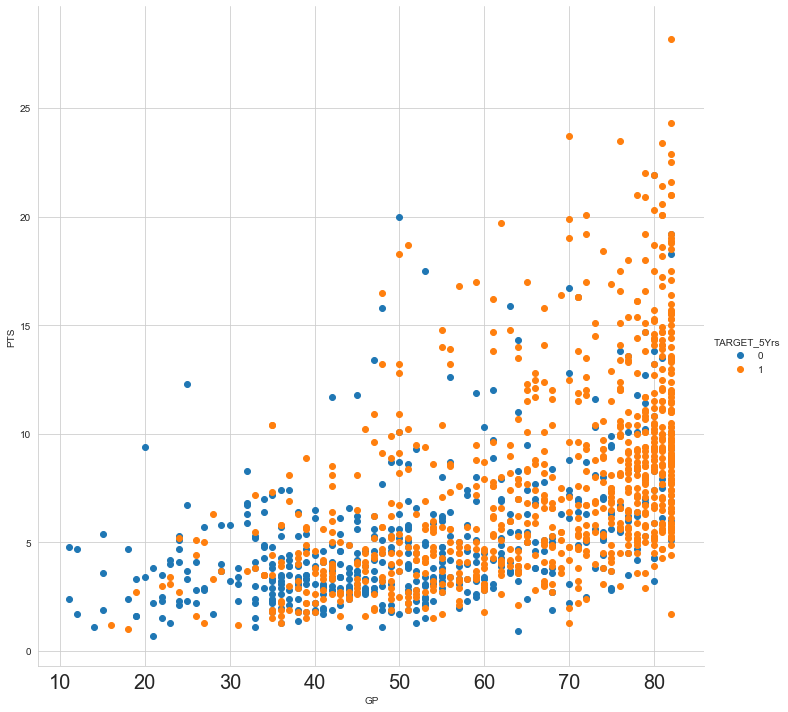
\includegraphics[scale=0.25]{model_1_scatter_plot.png}
    \caption{Model 1 scatter plot between independent and dependent variables}
    \label{fig:model1scatter}
\end{figure}
\begin{figure}[H]
    \centering
    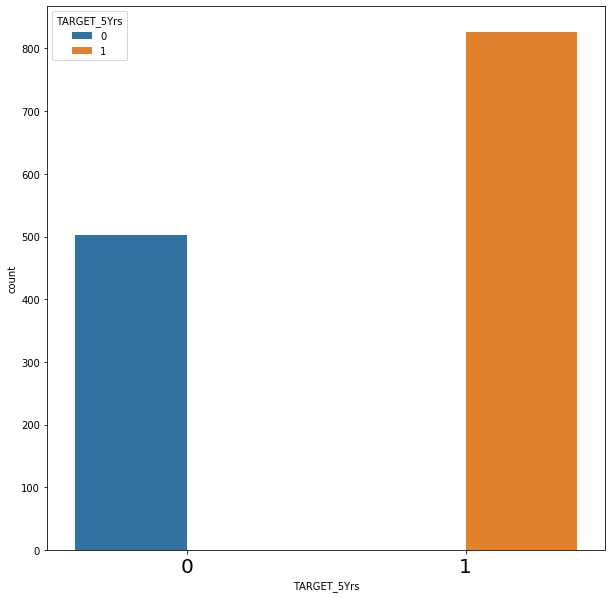
\includegraphics[scale=0.25]{model_1_bar_plot.png}
    \caption{Model 1 count plot for classes in response variable}
    \label{fig:model1bar}
\end{figure}
The model 2 performs predicting position in the basketball court based on the player's previous performance in the earlier regular 
seasons. The dataset used for this task is taken from \textit{basketball-reference.com} which consists of 47 attributes where 46 
attributes are independent variable and 1 variable is response variable and has over 10,000 rows of data. After performing the above 
mentioned pre-processing steps, the separability between independent variables and dependent variable was found using scatter plot
between games played and points earned coloured by response variable, see figure \ref{fig:model2scatter}.
\begin{figure}[H]
    \centering
    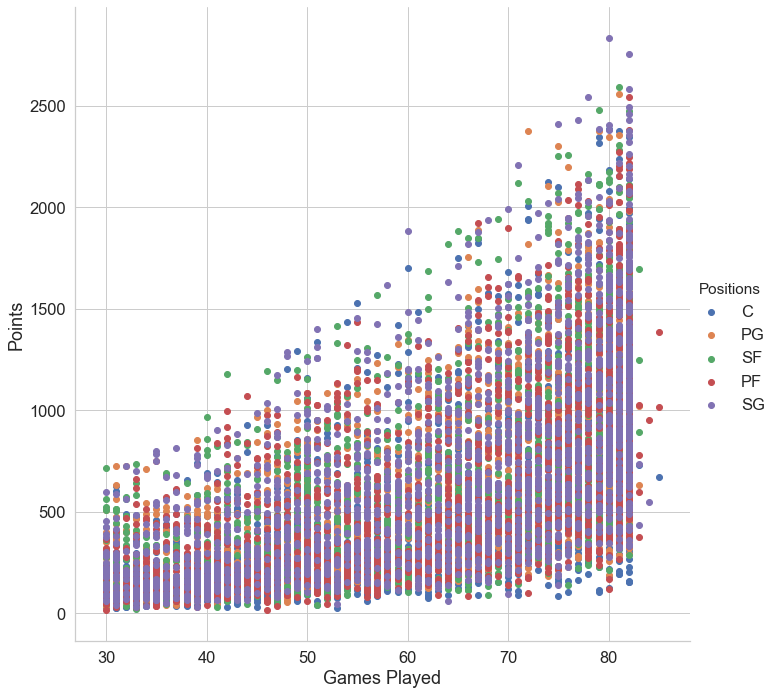
\includegraphics[scale=0.25]{model_2_scatter_plot.png}
    \caption{Model 2 scatter plot between independent and dependent variables}
    \label{fig:model2scatter}
\end{figure}
\begin{figure}[H]
    \centering
    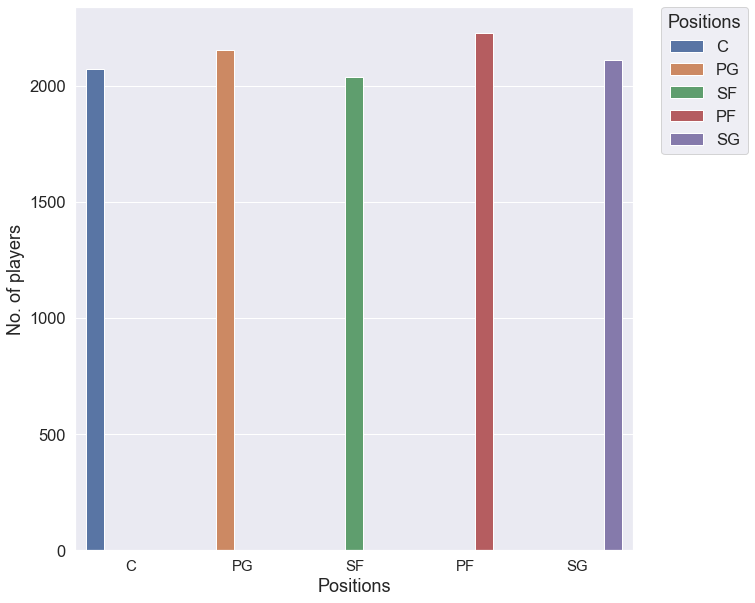
\includegraphics[scale=0.25]{model_2_bar_plot.png}
    \caption{Model 2 count plot for classes in response variable}
    \label{fig:model2bar}
\end{figure}
From the scatter plots, it can be observed that the data are not linearly separable. Moreover, it is not possible to create a classification 
boundary to separate data points that belong to differenct classes of the response variable. Hence, non-linear classification 
algorithms such as Support Vector Machine (SVM), K-Nearest Neighbor, and etc. has to be applied. Given the non-linear 
separability constraint and imbalanced dataset (model 1), see figure \ref{fig:model1bar}, it is best to choose Support Vector Machine (SVM) 
algorithm with kernel trick for both model 1 and model 2 because they train very well and yield good prediction results than other supervised learning 
algorithms \cite{imam2006z}. Before getting into detailed execution and discussion of test results, let us first understand about 
Support Vector Machine (SVM) algorithm.

Support Vector Machine (SVM) is one of the supervised learning algorithm used for classification, regression and outlier detection.
The objective of SVM is to find a hyperplane in N-dimensional space (N - number of attributes or features) which distinctly classifies
the data points, see figure \ref{fig:svm_1}.
\begin{figure}[H]
    \centering
    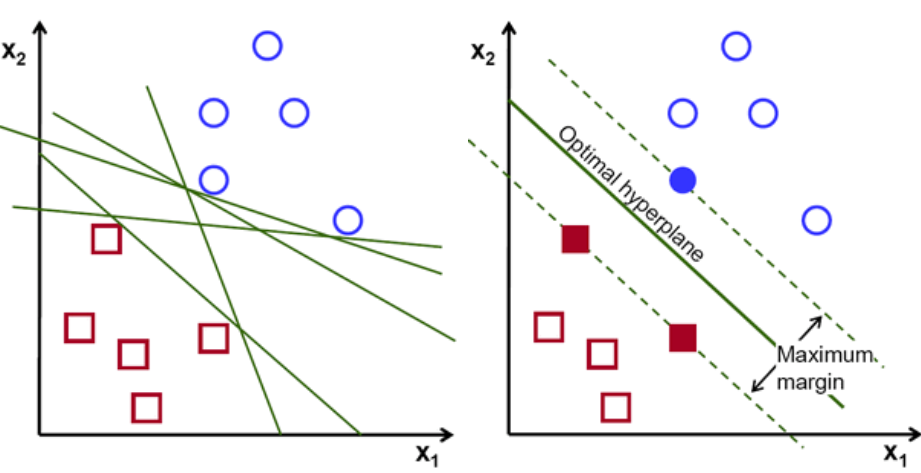
\includegraphics[scale=0.25]{svm_1.png}
    \caption{Hyperplane separating datapoints in N-dimesnional space}
    \label{fig:svm_1}
\end{figure}
From the above figure, we could see that to separate two classes of data points, there are many hyperplanes that could be chosen.
In order to choose the hyperplane that best separates the two classes of data points, we need to find \textit{maximum margin} - the
maximum distance between data points of both classes. Let us now look at hyperplanes and support vectors followed by maximum margin.

Hyperplanes are classification boundary that separated data points. Data points falling to either side of the hyperplane are 
attributed to different classes. The dimension of hyperplane depends on the number of input features, that is, if the number of 
input feature is 2, then the hyperplane is a line, see figure \ref{fig:svm_hyperplane_1}. If the number of input feature is 3, then 
the hyperplane becomes two dimensional plane, see figure \ref{fig:svm_hyperplane_2}. It might not be possible to imagine, if the 
number of features exceeds 3.

\begin{figure}[H]
    \centering
    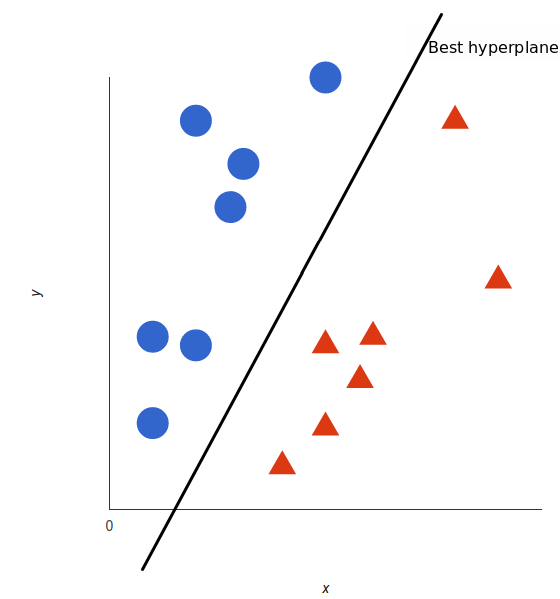
\includegraphics[scale=0.25]{svm_hyperplane_1.png}
    \caption{Hyperplane in 1-dimesnional space}
    \label{fig:svm_hyperplane_1}
\end{figure}
\begin{figure}[H]
    \centering
    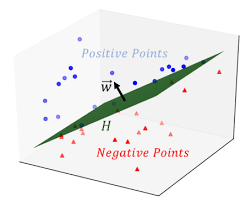
\includegraphics[scale=0.60]{svm_hyperplane_2.png}
    \caption{Hyperplane in 2-dimesnional space}
    \label{fig:svm_hyperplane_2}
\end{figure}

Support vectors are data points which are closer to the hyperplane. The orientation and position of hyperplane are decided by 
these support vectors. The margin of the classifier is maximized using these support vectors. In SVM, we are trying to maximize 
the distance between the data points and hyperplane which is achieved by applying a loss function - \textit{Hinge Loss}. The intuition
behind maximizing the margin is to avoid \textit{misclassification} of data points, that is, if we have made a mistake in placing 
the boundary, then the model will not generalize well on unforseen data. Moreover, maximizing the margin avoids local minima
\cite{jakkula2006tutorial}. 

The equation for hyperplane in P-dimension is given below.
\begin{figure}[H]
    \centering
    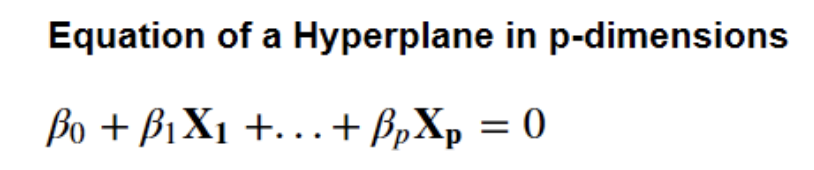
\includegraphics[scale=0.40]{SVM_Equation_for_p-dimension.png}
    \caption{Equation for P-dimesnional space}
    \label{fig:svm_dimension_equation}
\end{figure}

Where the datapoints are, see figure \ref{fig:svm_datapoints},
\begin{figure}[H]
    \centering
    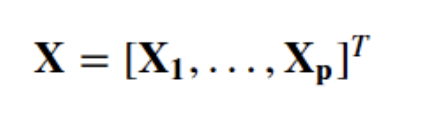
\includegraphics[scale=0.40]{svm_data_points.png}
    \caption{Equation for P-dimesnional space}
    \label{fig:svm_datapoints}
\end{figure}

and the datapoints are classified into different classes based on the below equation, see figure \ref{fig:classification}
\begin{figure}[H]
    \centering
    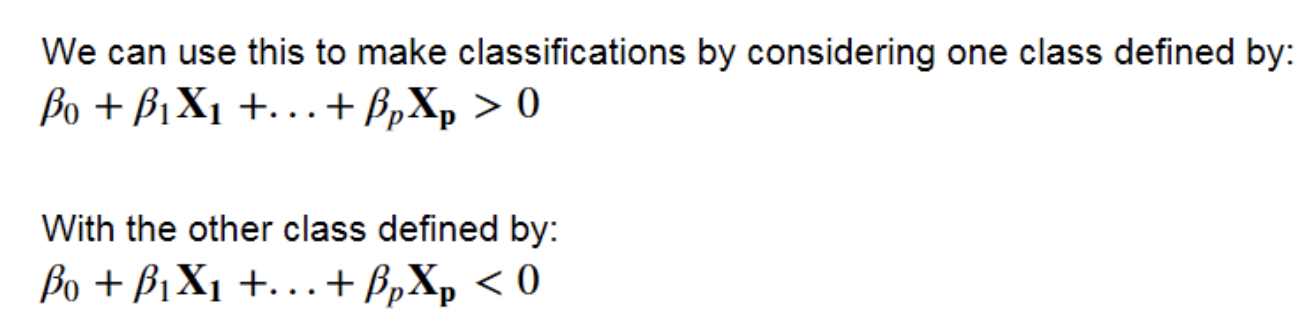
\includegraphics[scale=0.40]{dimension_equation_for_classification.png}
    \caption{Equation for classifying data points}
    \label{fig:classification}
\end{figure}
Now, we understand that data which are not linearly separable are projected to higher dimensions and classified, but it may not be 
easy to perform this, if the number of features increase. It would be computationally expensive to project large dimesnional data
to higher dimensions. This where \textit{Kernel Trick} is applied in order to resolve this problem \cite{kernel}. For model 1 and 
model 2, the number of features are high in number and the data is not linearly separable. Hence, SVM kernel trick has to be used
to solve the task of classifying players and predicting positions of players. "The trick is that kernel methods represent the data 
only through a set of pairwise similarity comparisons between the original data observations x (with the original coordinates in the 
lower dimensional space), instead of explicitly applying the transformations $\phi(x)$ and representing the data by these 
transformed coordinates in the higher dimensional feature space" \cite{kernel}. There are many kernels available in SVM namely
\textit{Linear}, \textit{polynomial}, \textit{Radial Base Function (RBF)}, and \textit{sigmoid}. From the list of aforementioned kernels, only polynomial
and rbf kernel methods can be applied to our data. Before choosing the kernel method that best suits our data, we need to understand
some hyperparameters such as gamma, and C.
\begin{itemize}
    \item Gamma - inverse of the standard deviation of the RBF kernel (Gaussian function), which is used as similarity measure between two points
    \cite{scikitlearn}.
    \item C - Penalty factor for misclassification. \cite{scikitlearn}.
\end{itemize}
The best kernel method is chosen by performing \textit{GridSearch Cross Validation} with various values for aforementioned hyperparameters.
This method provides the hyperparameters with values and kernel method which generalizes well on unforseen data. Based on the 
values provided by GridSearch method, the models are trained by using SVM function from sklearn library on a part of data and tested 
on remaining part of the data. The test results of the models are explained in the forthcoming sections.

Finally, model 3 performs clustering or grouping of players into groups based on their previous performances. This is an unsupervised
machine learning task where the dataset does not contain labels for prediction or grouping. The dataset used for this task is taken from 
\textit{basketball-reference.com} which consists of 47 attributes where 46 attributes are independent variable and 1 variable is 
response variable and has over 28,000 rows of data. Data was grouped by players and fileterd based on the number of games played by players 
is greater than 30 after performing the above mentioned pre-processing steps because data with games played less than 30 will not provide 
meaningful insight. There were 3 features missing from the data namely FT\% - Free Throw percentage, 2P\% - 2 Point percentage, and
3P\% - 3 Point percentage which were created by applying feature engineering, that is, creating new features with available data 
points. The simplest form of clustering is the partitional clustering which aims at partitioning the given data into set of disjoint
subsets (clusters). The most commonly used clustering criterion is \textit{clustering error} which measures the quality of clustering.
A popular clustering method that minimizes the clustering error is the k-means algorithm \cite{likas2003global}. Hence, K-means 
clustering algorithm would be a good technique to cluster the players. Moreover, in K-means we can specify the number of clusters 
we require which is an added advantage. Before getting into detailed execution and discussion of test results, let us first understand about 
K-means algorithm.

K-means algorithm is one of the unsupervised algorithm mainly used for clustering of unlabelled data. A good clustering solution 
is one that finds clusters such that the observations within each cluster are more similar than the clusters themselves, see figure
\ref{fig:kmeans}.
\begin{figure}[H]
    \centering
    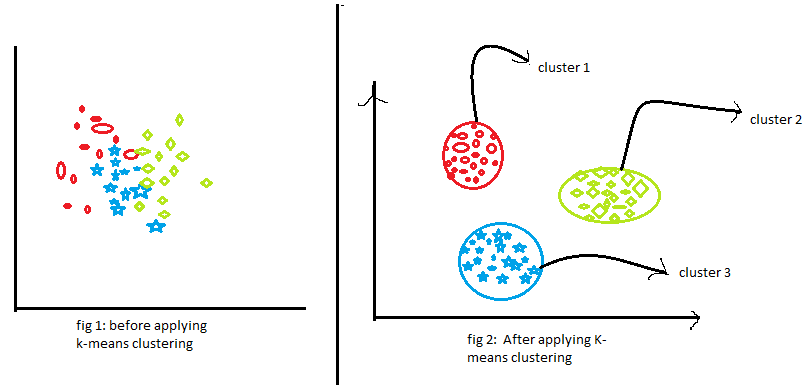
\includegraphics[scale=0.45]{kmeans.png}
    \caption{K-means clustering}
    \label{fig:kmeans}
\end{figure}
The process behind K-means algorithm is very simple. Firstly, we need to choose an appropriate value for "K". Secondly, we need to 
randomly choose an initial centroid (centre coordinates) for each cluster, then we need apply two step process which is given below,
\begin{itemize}
    \item Assignment step - Assign each data point to it's nearest centre.
    \item Update step - Update the centroids as being the centre of of their observation.
\end{itemize}
We repeat these steps over and over until there is no further change in the clusters. At this point the algorithm converges and 
we retrieve the final clusterings. Every data point is assigned to each of the clusters thus reducing the incluster sum of squares.
In other words, K-means identifies K centroids and allocates the data points to each K centroids while keeping the centroid as small
as possible \cite{kmeans}. 

The pictorial representation of working of K-means algorithm, see figure \ref{fig:kmeansworking},
\begin{figure}[H]
    \centering
    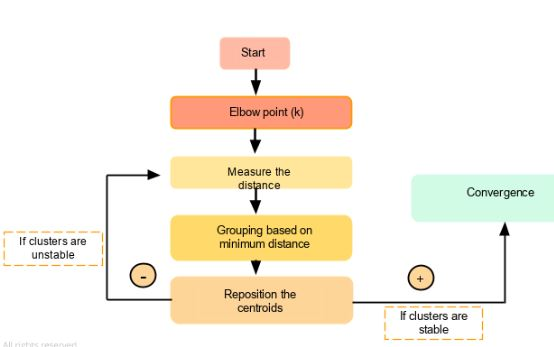
\includegraphics[scale=0.55]{kmeans_1.jpeg}
    \caption{Working of K-means clustering}
    \label{fig:kmeansworking}
\end{figure}

The value of "K" is determined by two methods namely \textit{Elbow method} and \textit{Silhouette score}. However, elbow method is 
the most commonly used to determine K value. The elbow method runs the K-means algorithm on the dataset for various K values, then
for each K value computes the average score for all clusters and stores. When these values are plotted to visually determine the best 
value for K. If the line chart looks like an arm, then the “elbow” (the point of inflection on the curve) is the best value of k. 
The “arm” can be either up or down, but if there is a strong inflection point, it is a good indication that the underlying model 
fits best at that point \cite{elbow}. The pictorial representation of choosing K using elbow method, see figure \ref{fig:elbowmethod}.
The test results of this model is explained in the forthcoming sections.
\begin{figure}[H]
    \centering
    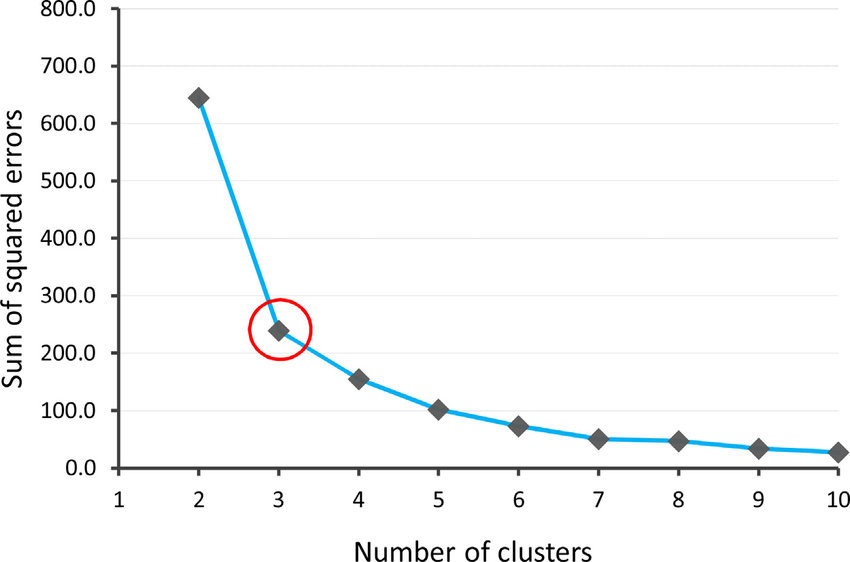
\includegraphics[scale=0.25]{elbow_method.png}
    \caption{Elbow Method}
    \label{fig:elbowmethod}
\end{figure}

\subsection{Evaluation Metrics}
\hfill\\
In the field of machine learning there are several measures to know the quality and characteristics of a model. The most commonly used
evaluation metrics for classification task are \textit{Accuracy}, \textit{Recall}, \textit{Precision}, \textit{F1 score} and 
\textit{Receiver Operating Characteristic (ROC) curve}. The evaluation metrics used for regression task are 
\textit{Adjusted R\textsuperscript{2}}, \textit{Mean Squared Error(MSE)}, \textit{Root-Mean-Squared-Error(RMSE)}, and etc. 
The evaluation metrics used for clustering tasks are \textit{Silhouette Coefficient} and \textit{Dunn's index} 
\cite{powers2020evaluation}. In this project, we are going to use the evaluation metric for classification and clustering alone. 
Let us first understand about each evaluation metric before reading further.

Evaluation of the performance of a classification model is based on the counts of test records correctly and incorrectly predicted 
by the model. The confusion matrix, see figure \ref{fig:confusionmatrix} which provides a more insightful picture which is not only the 
performance of a predictive model, but also which classes are being predicted correctly and incorrectly, and what type of errors 
are being made \cite{confusionmatrix}.

\begin{figure}[H]
    \centering
    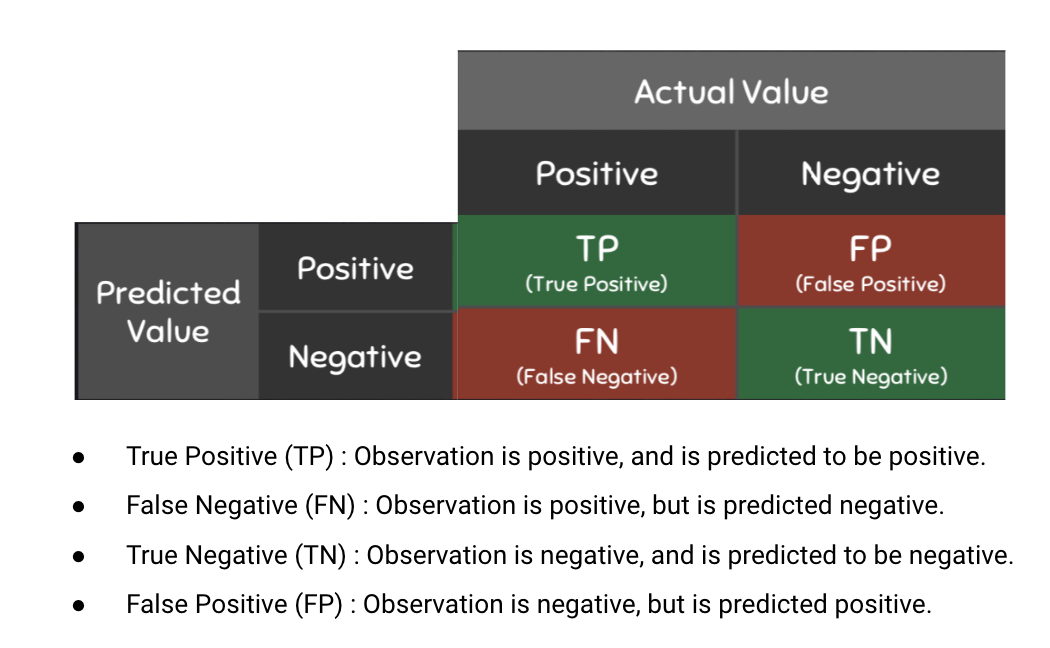
\includegraphics[scale=0.22]{confusion_matrix.png}
    \caption{Confusion Matrix}
    \label{fig:confusionmatrix}
\end{figure}
\hfill\\
\textbf{Accuracy}: In general, the accuracy metric measures the ratio of correct predictions over the total
number of instances evaluated \cite{hossin2015review}, see figure \ref{fig:aprf} for formula. \\
\textbf{Recall}: Recall is used to measure the fraction of positive patterns that are correctly classified \cite{hossin2015review}, 
see figure \ref{fig:aprf} for formula. \\
\textbf{Precision}: Precision is used to measure the positive patterns that are correctly predicted from the total predicted 
patterns in a positive class \cite{hossin2015review}, see figure \ref{fig:aprf} for formula. \\ 
\textbf{F1 Score}:This metric represents the harmonic mean between recall and precision values \cite{hossin2015review}, see figure 
\ref{fig:aprf} for formula. \\
\begin{figure}[H]
    \centering
    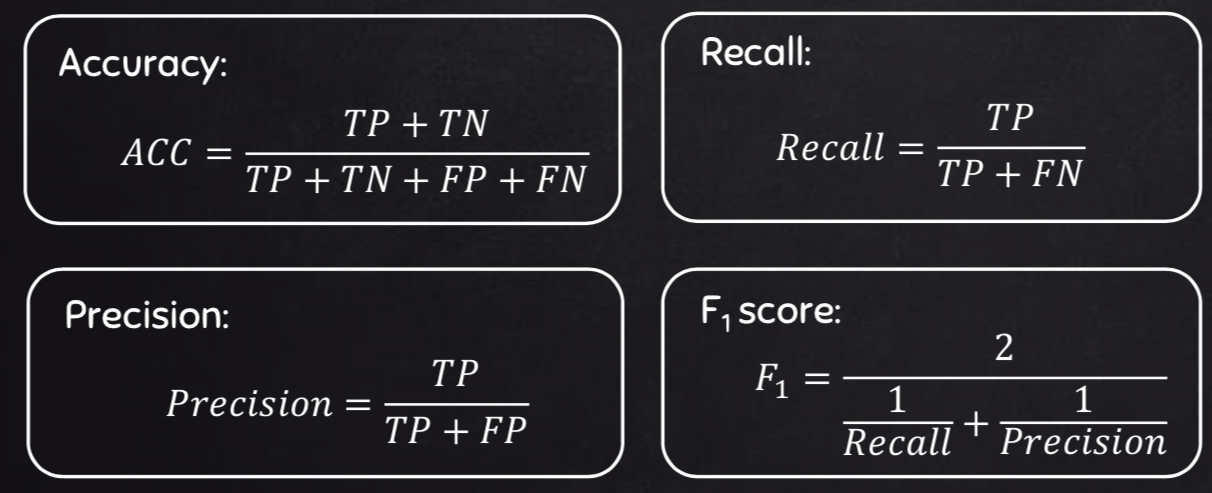
\includegraphics[scale=0.18]{evaluation_metrics_for_classification.png}
    \caption{Accuracy, Precision, Recall and F1 Score}
    \label{fig:aprf}
\end{figure}

\textbf{ROC Curve}:ROC is a major visualization technique for presenting the performance of a classification model. 
It summarizes the trade-off between the \textit{true positive rate (tpr)} and \textit{false positive rate (fpr)}, see figure \ref{tprfpr} 
for a predictive model using different probability thresholds \cite{confusionmatrix}.
\begin{figure}[H]
    \centering
    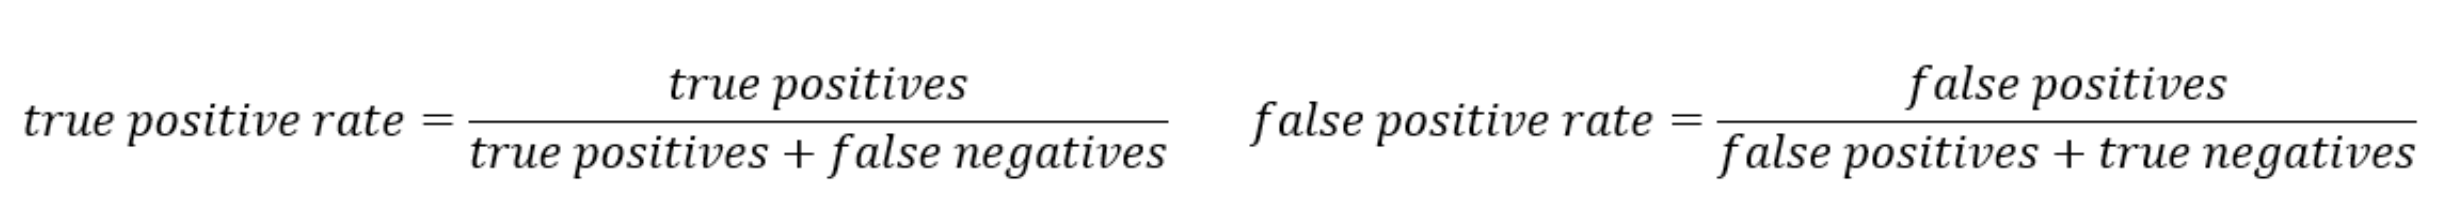
\includegraphics[scale=0.18]{tpr_fpr_equation.png}
    \caption{Equation of tpr and fpr}
    \label{fig:tprfpr}
\end{figure}
A ROC curve, see figure \ref{fig:roc}, plots the true positive rate (tpr) versus the false positive rate (fpr) as a function of the 
model’s threshold for classifying a positive. Finally, we can assess the performance of the model by the area under the ROC 
curve (AUC). As a rule of thumb, 0.9–1 = excellent; 0.8-.09 = good; 0.7–0.8 = fair; 0.6–0.7 = poor; 0.50–0.6 = fail 
\cite{confusionmatrix}.
\begin{figure}[H]
    \centering
    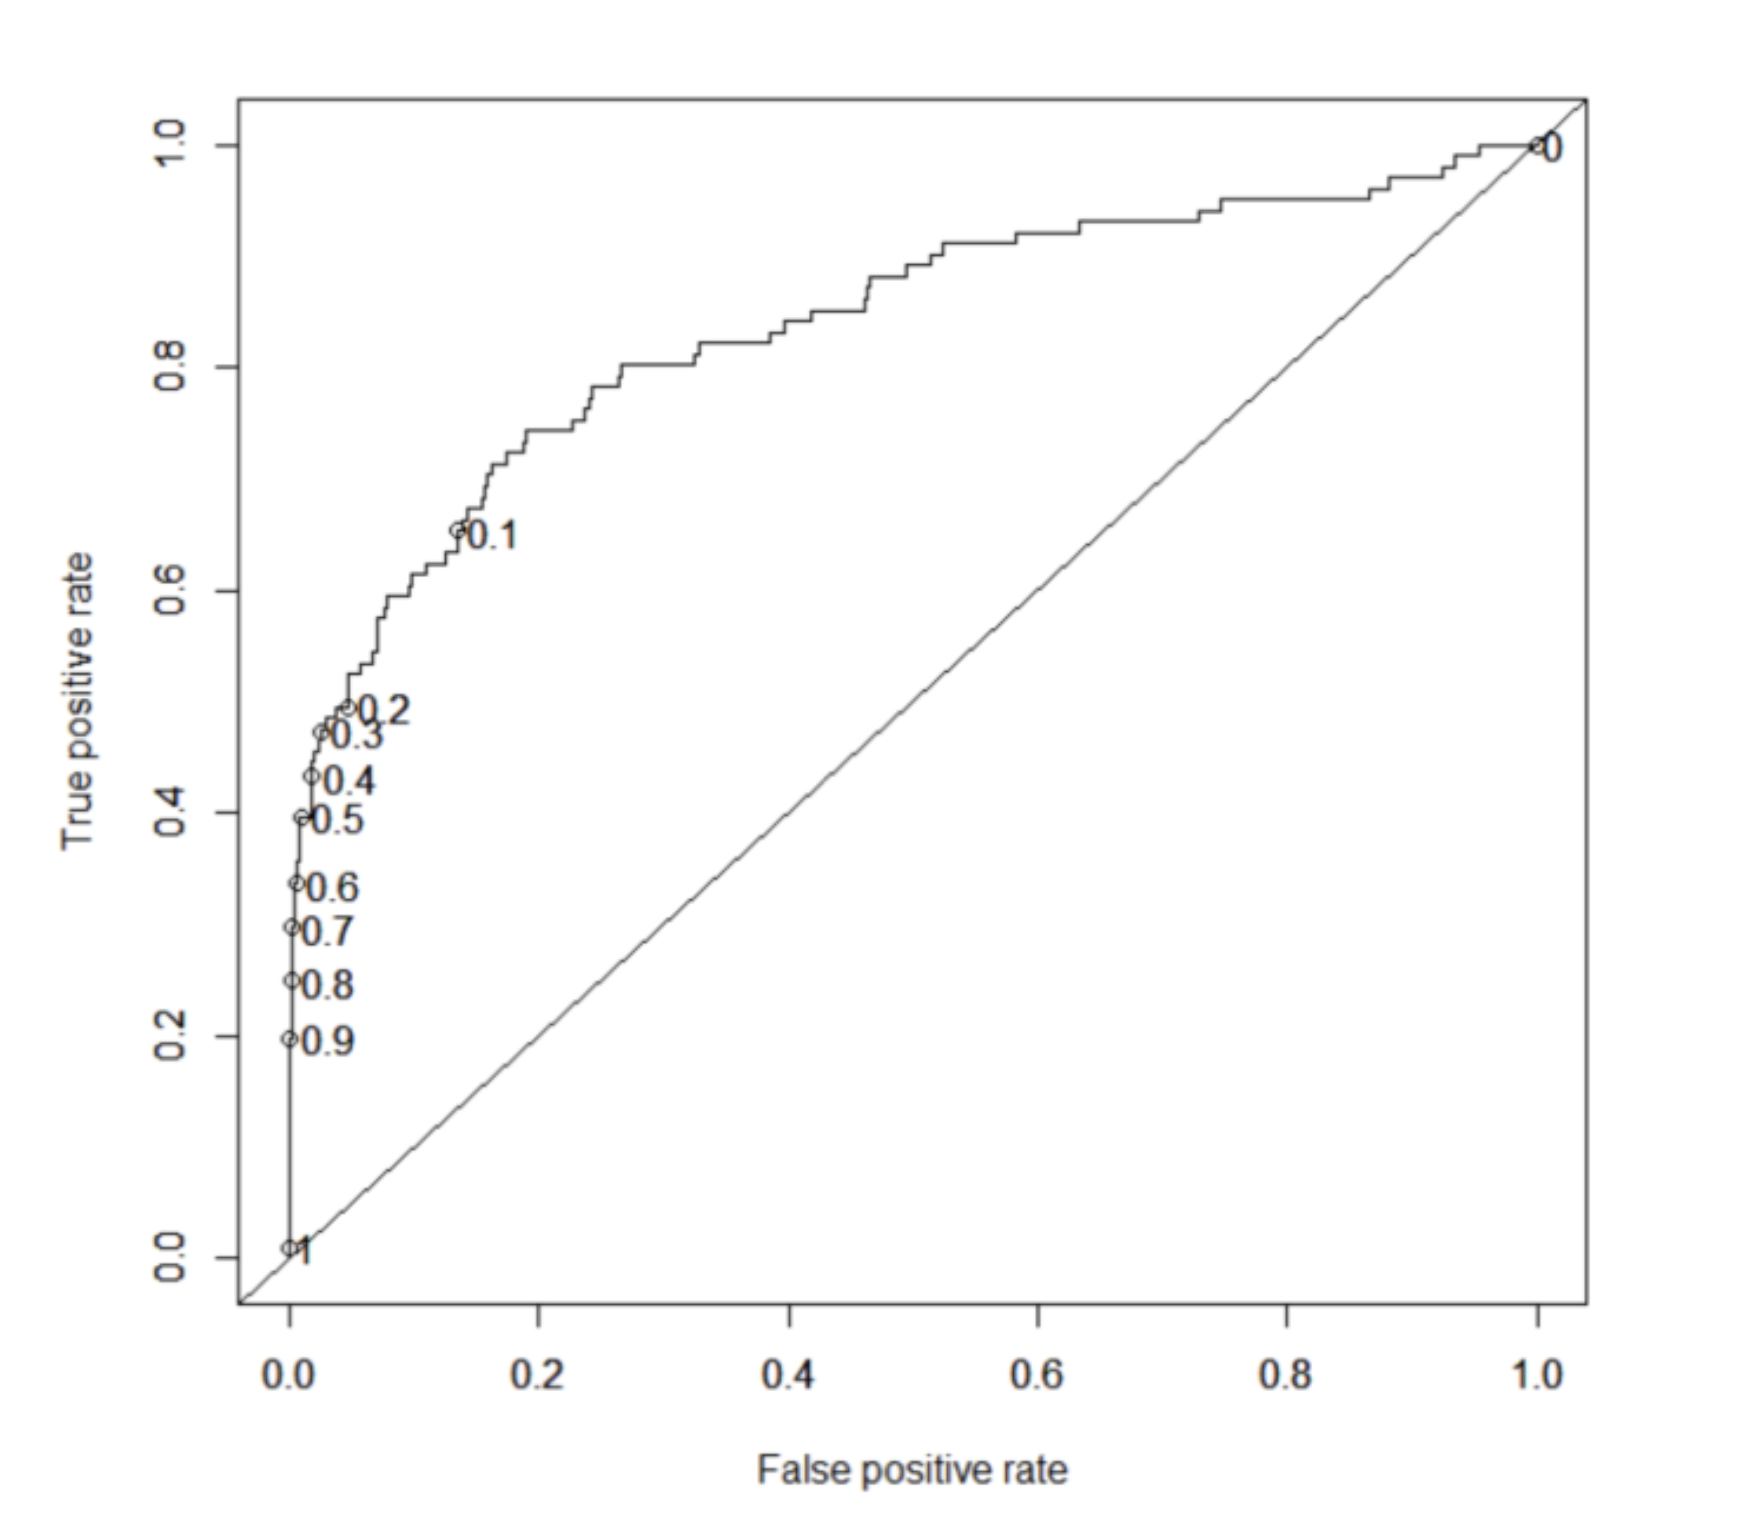
\includegraphics[scale=0.25]{AUC_ROC_Curve.png}
    \caption{ROC Curve}
    \label{fig:roc}
\end{figure}
Clusters are evaluated based on some similarity or dissimilarity measure such as the distance between cluster points. 
If the clustering algorithm puts the data points of similar distance together and disimilar points away from the cluster, 
then it has performed well. The aforementioned two metrics for clustering algorithm is given below,

\textit{\textbf{Silhouette Coefficient}}\\
\begin{figure}[H]
    \centering
    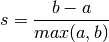
\includegraphics[scale=0.60]{silhouette_coefficient.png}
    \caption{Silhouette Coefficient}
    \label{fig:silc}
\end{figure}

The silhouette coefficient consists of two scores in the above formula where, 
\begin{itemize}
    \item a - The mean distance between a sample and all other points in the same cluster.
    \item b - The mean distance between a sample and all other points in the next nearest cluster.
\end{itemize}
For each sample, mean silhouette coefficient is calculated and if the value is bound between -1, then it is incorrect clustering. If
the value is bound between 1, then it is correct clustering. If the value is around zero, then it is overlapping clusters \cite{evaluationmetric}.

\textit{\textbf{Dunn's Index}} \\
Dunn’s Index is equal to the minimum inter-cluster distance divided by the maximum cluster size. 
Large inter-cluster distance = better separation, smaller inter-cluster distance = more compact cluster leading to high Dunn's index
value. A higher Dunn’s index score represents better clustering \cite{evaluationmetric}. 
\bibliographystyle{ACM-Reference-Format}
\bibliography{references}
\end{document}

